\chapter{GPU Computing}
\label{sec:gpu}


L'obiettivo di questo capitolo è presentare i concetti fondamentali dei sistemi eterogenei e della programmazione GPU, con particolare attenzione ai framework CUDA e Vulkan. Ottenere una visione approfondita di tali concetti contribuirà a una migliore comprensione delle scelte tecnologiche e dei dettagli implementativi discussi nel capitolo del progetto finale. Il capitolo è diviso in due senzioni: la prima si concentra sul modello di programmazione GPGPU, mentre la seconda fornirà un'analisi dettagliata di CUDA e Vulkan per lo sviluppo di software.

\section[General-purpose computing su GPU]{General-purpose computing su GPU}

Sebbene le CPU e le GPU siano entrambi processori che eseguono istruzioni macchina, esse si differenziano soprattutto nell'approccio usato nell'eseguire programmi paralleli: mentre le CPU multi-core possono adottare un approccio di tipo Multiple Instruction Multiple Data (MIMD) o Single Instruction Multiple Data (SIMD), le GPU seguono un modello di istruzioni Single Instruction Multiple Thread (SIMT), in cui il carico di lavoro è suddiviso in sottoproblemi risolvibili singoli thread indipendent. Lo sviluppo delle GPU si è storicamente concentrato nell'ambito delle industria dei videogiochi, il cui impegno tecnologico è sempre stato finalizzato a offrire esperienze virtuali il più realistiche possibili. Per raggiungere questo obiettivo, sono richiesti un numero considerevole di calcoli geometrici (come rotazioni e traslazioni), tipicamente sotto forma di operazioni in virgola mobile, per ogni pixel dello schermo. Le GPU sono state concepite appositamente come dispositivi ottimizzati per computazioni altamente parallele, come nel caso del rendering grafico. Le architetture delle GPU sono strutturate seguendo il modello many-thread anziché multi-core, mettendo quindi l'accento sull'ottimizzazione del trattamento dei dati piuttosto che sulla memorizzazione e sul controllo del flusso dei dati.
Entrambi i modelli sono rappresentati in fig. \ref{fig:cpu_vs_gpu}.

\begin{figure}[ht]
    \centering
    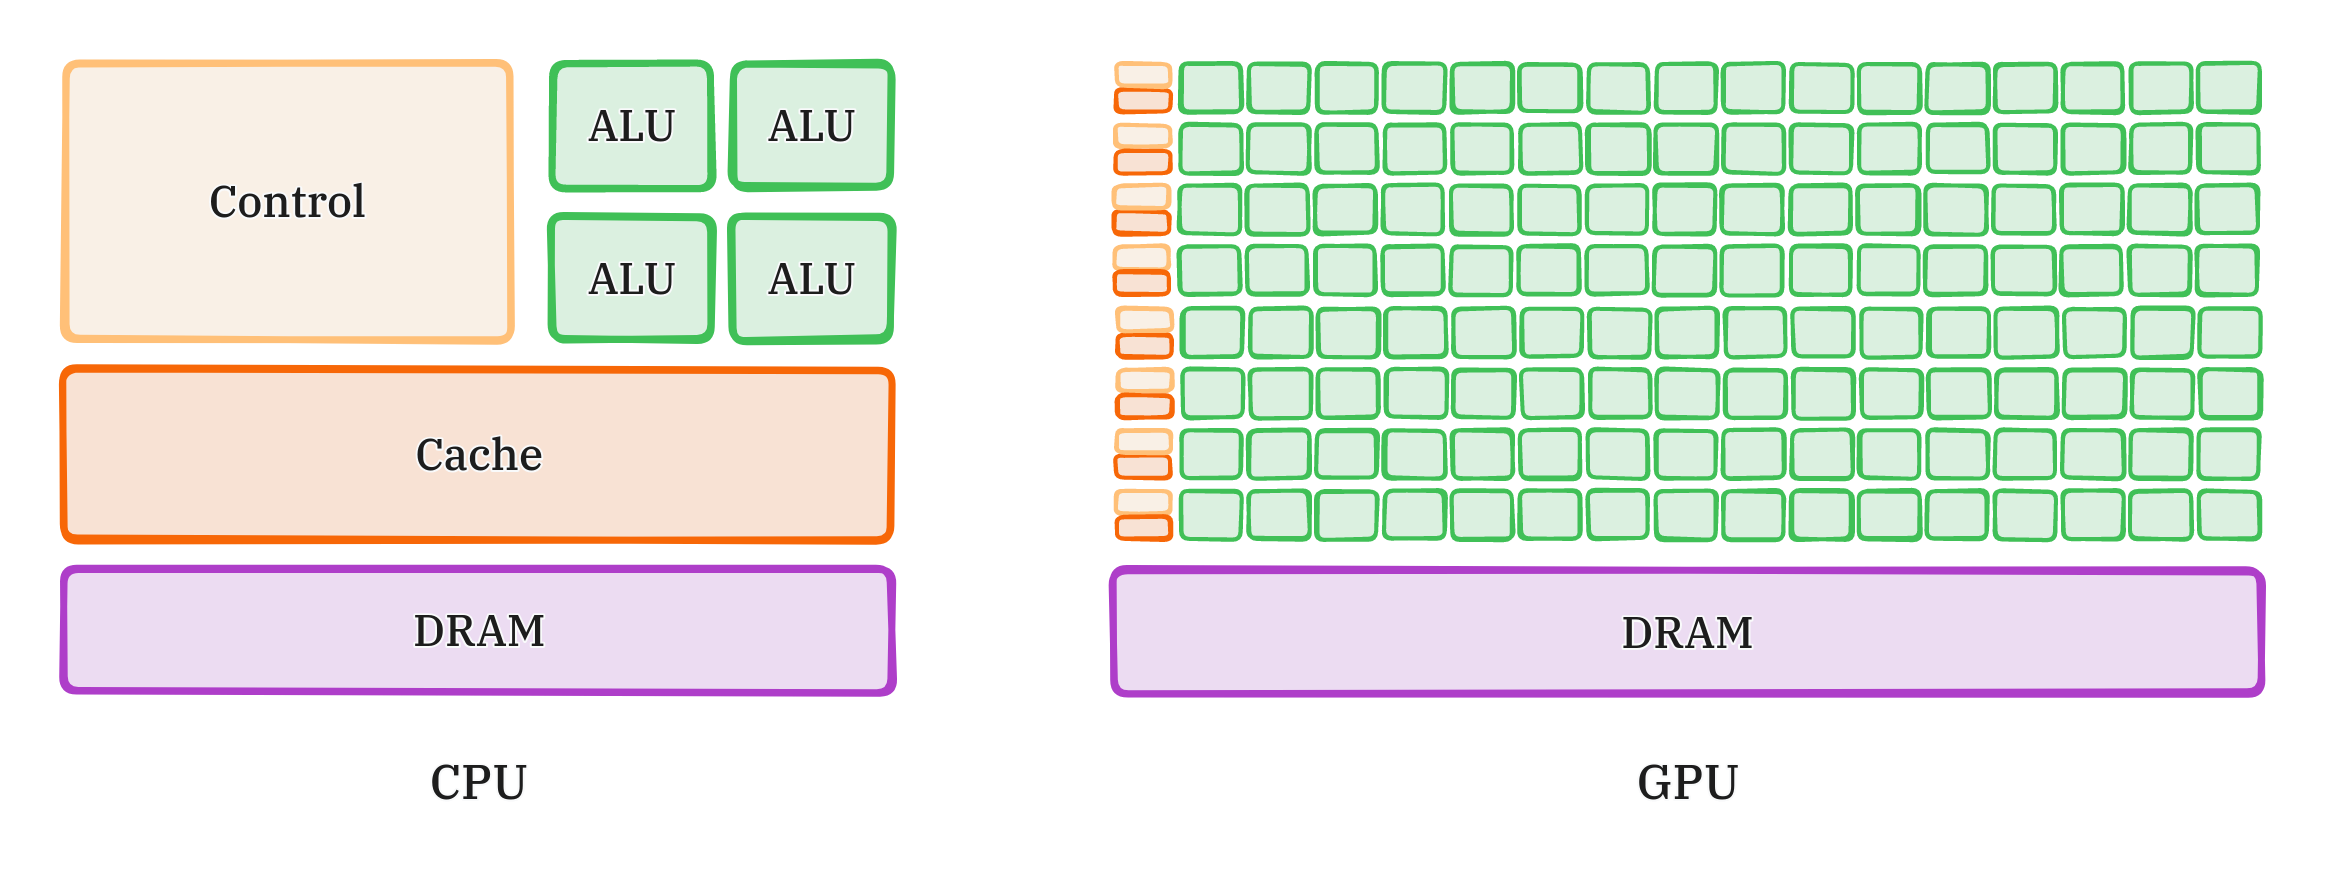
\includegraphics[width=.9\linewidth]{images/chapter2/cpu_vs_gpu.png}
    \caption{Confronto fra l'architettura CPU e GPU}
    \label{fig:cpu_vs_gpu}
\end{figure}

Usare le prime GPU per il computing era molto difficile, perché gli sviluppatori erano costretti a usare le API grafiche per accedere ai core del processore. Ciò significava che un calcolo doveva essere espresso come una funzione che colora un pixel in modo tale da venir eseguito dall'hardware. Questa tecnica era comunemente usata gli albori della GPGPU. Anche con un ambiente di programmazione di alto livello, il codice sottostante doveva ancora adattarsi alle API progettate per colorare i pixel, che limitavano i tipi di applicazioni che si potevano effettivamente sviluppare e, conseguentemente, impedivano il diffondersi di questa tecnologia.
Il paradigma di GPGPU consente di sfruttare la potenza di calcolo delle GPU non solo per la grafica dei videogiochi, ma anche per eseguire calcoli generici di natura scientifica ed ingegneristica, come l'ottimizzazione nella simulazione di sistemi fisici reali. Grazie alla GPGPU, il trasferimento di dati tra CPU e GPU diventa bidirezionale e, di conseguenza, in sistemi che richiedono numerose operazioni su grandi quantità di dati si può osservare un notevole miglioramento delle prestazioni. Un'implementazione intelligente del paradigma SIMD su GPU può conseguire un aumento di velocità fino a 100 volte rispetto a un'implementazione sequenziale su un singolo core CPU. Secondo la tassonomia di Flynn (!!TODO aggiungere ref), un sistema è classificato come SIMD (Single Instruction Multiple Data) se esegue una singola istruzione, o anche un piccolo insieme di istruzioni, in parallelo su un vasto numero di dati. Il paradigma SIMT è simile, e affida l'esecuzioni di un ristretto insieme di istruzione a un singolo thread, sarà poi compito del programmatore aggregare i risultati di ogni thread GPU e ottenere la computazione finale.

In genere, un sistema non può essere parallelizzato in tutte le sue parti, limitando l'accelerazione delle prestazioni a una piccola porzione del codice. Pertanto, è necessario progettare sistemi in cui alcune parti siano concepite in parallelo, mentre altre in modo sequenziale. Per questo motivo, nel modello GPGPU, CPU e GPU collaborano tra loro, dando origine a un modello di elaborazione eterogenea in cui la CPU gestisce la parte sequenziale, mente la GPU esegue in parallelo la parte comutazionalmente onerosa.
La fig. \ref{fig:het_model} mostra il modello di un sistema eterogeneo: il carico di lavoro parallelizzabile, è affidato alla GPU, mentre il compito di gestire i processi e la suddivisione in sottoproblemi è affidata alla CPU.

\begin{figure}[ht]
    \centering
    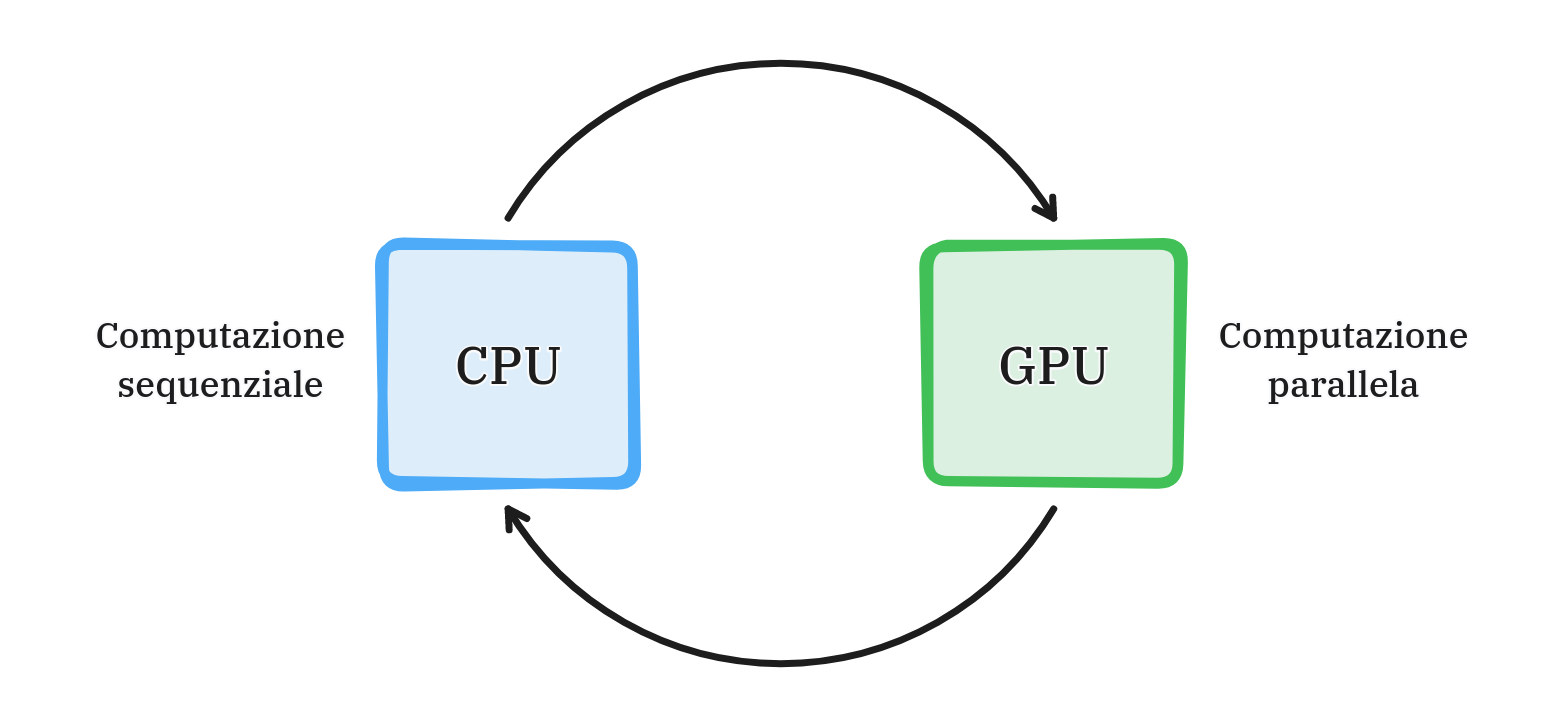
\includegraphics[width=.9\linewidth]{images/chapter2/het_model2.png}
    \caption{Modello di un sistema eterogeneo}
    \label{fig:het_model}
\end{figure}


Inizialmente, le GPU e i linguaggi di programmazione parallela erano destinati a un mercato molto diverso rispetto alle CPU. Nella programmazione ``classica'' delle CPU, la compatibilità tra diverse versioni dello stesso software è stata fin dall'inizio un requisito fondamentale, mentre l'innovazione in termini di miglioramento delle GPU ha spesso comportato cambiamenti drastici nell'hardware. Queste evoluzioni tecnologiche hanno portato a una perdita di portabilità tra i diversi modelli: l'introduzione di nuove tecnologie hardware ha portato a proposte di architetture GPU completamente nuove, con significative differenze tra loro. Di conseguenza, queste nuove architetture richiedevano quasi sempre una ridefinizione completa dei relativi codici. Si è rilevato quindi necessario stabilire degli standard operativi per poter, quantomeno, mantenere un modello logico coerente tra le diverse architetture.
I principali standard per l'elaborazione parallela sono MPI, OpenMP.

\begin{itemize}
    \item \textbf{MPI}: progettato per sistemi di memoria distribuita, utilizzato in ambienti di HPC in cui più processori o nodi comunicano scambiandosi messaggi. Solitamente viene usato per l'architettura di supercomputer, nei queli migialia di nodi sono connessi attraverso una rete dedicata. Ogni problema viene suddiviso in diversi sottoproblemi, ognuno dei quali è risolto da un nodo specifico. Questo modello è poco flessibile e oneroso di risorse e soprattutto una rete dedicata molto veloce che si possa far carico dei messaggi tra i nodi.
    \item \textbf{OpenMP}: offre un insieme di direttive del compilatore e routine di libreria per il multiprocessing su singole macchine a memoria condivisa, comunemente usato per parallelizzare cicli e altre regioni di codice per sfruttare i processori multi-core. Dato che il software deve essere eseguito sulla stessa macchina questo modello è relativamente più semplice del precedente, ma limitato dal punto di vista prestazionale.
\end{itemize}

\begin{figure}[ht]
    \centering
    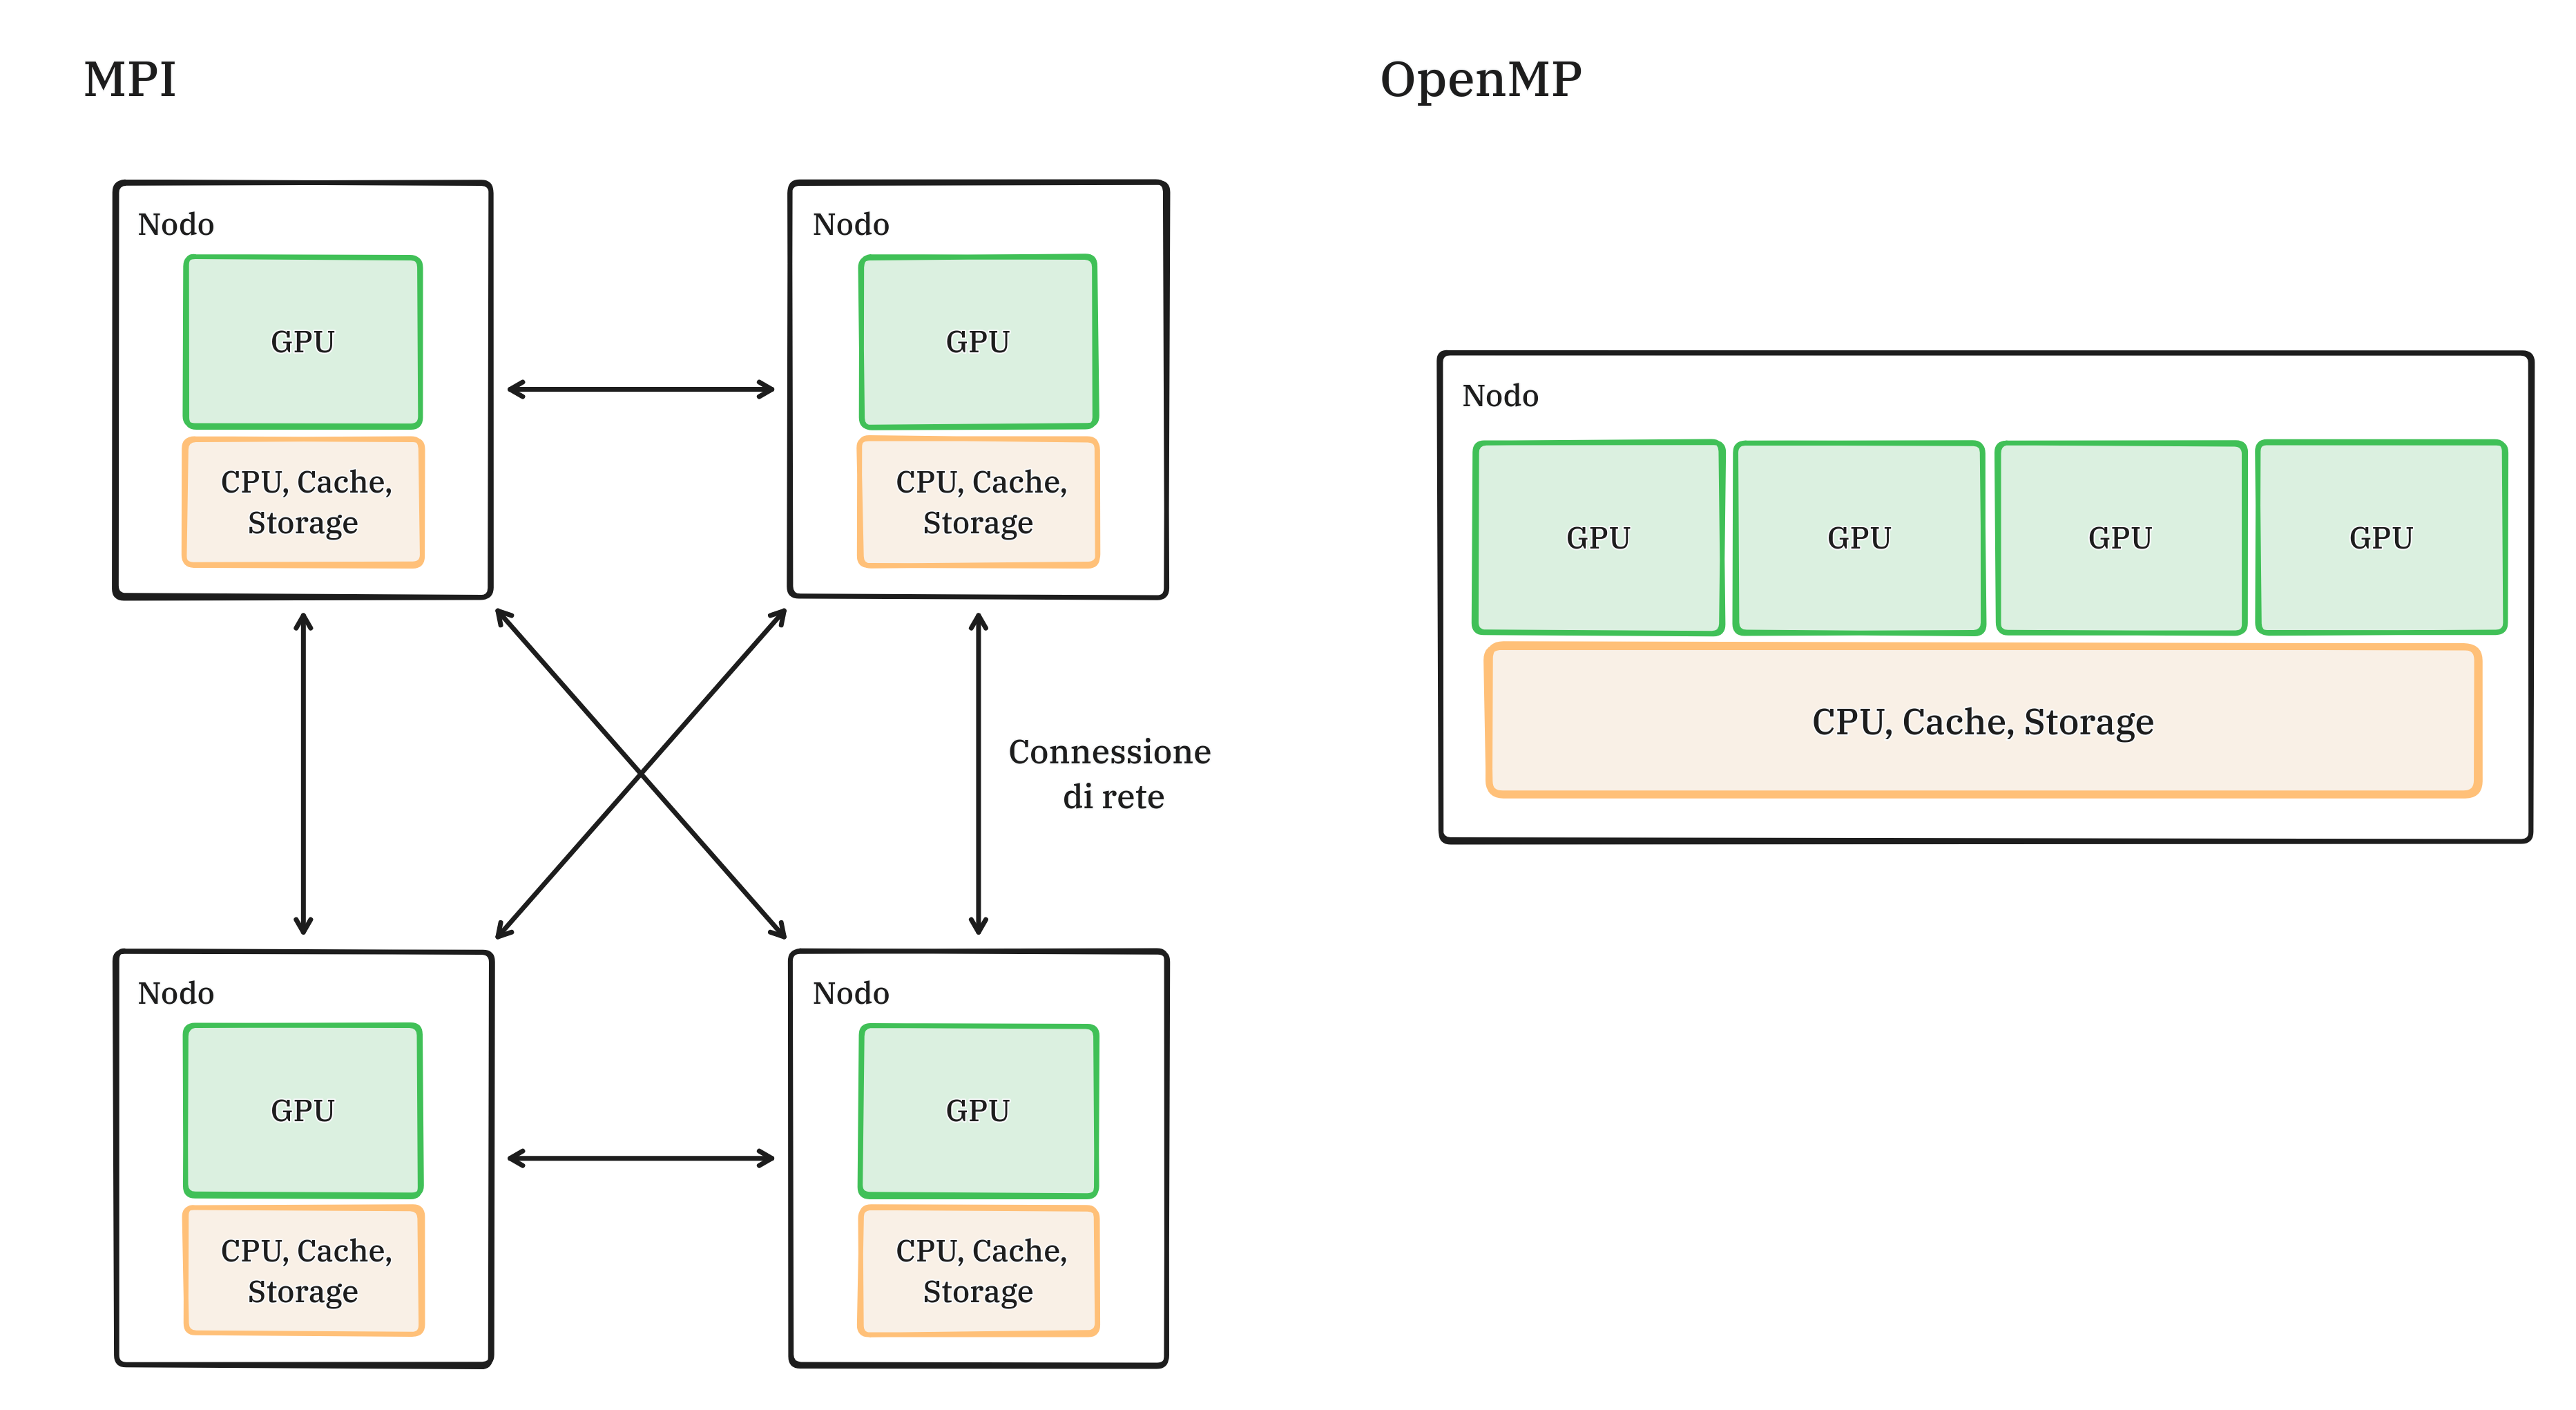
\includegraphics[width=.9\linewidth]{images/chapter2/mpi_openmp.png}
    \caption{Sistema MPI e OpenMP a confronto}
    \label{fig:mpi_openmp}
\end{figure}

Il modello OpenMP consente al programmatore di raggiungere un alto livello di parallelizzazione, specificando, in modo semplice ,le porzioni specifiche del codice da ottimizzare. D'altra parte, in MPI i nodi non condividono la memoria e tutti i dati sono condivisi attraverso messaggi, garantendo elevata scalabilità anche su centinaia di miglia di nodi; implementarlo, però,  può risultare difficile proprio per la mancanza di memdoia condivisa tra i nodi. A causa della loro natura intrinsecamente diversa, è raro utilizzare contemporaneamente questi standard. In fig. \ref*{fig:mpi_openmp} è mostata la sostanziale differenza tra i due modelli.

Con l'introduzione di CUDA, NVIDIA ha fornito agli sviluppatori un framework in grado di combinare i vantaggi dei due standard. Con l'acronimo CUDA, che sta per Compute Unified Device Architecture, si intende non solo il linguaggio di programmazione, ma anche l'architettura hardware. Per sfruttare appieno questo framework, è necessaria una GPU compatibile con CUDA e, dato che è sviluppato da NVIDIA, tutte le loro GPU recenti lo supportano. L'architettura tipica di una GPU NVIDIA compatibile con CUDA è illustrata in fig. \ref{fig:cuda_arch}. Le differenze tra i vari modelli possono essere negli Streaming Multiprocessors (SMs) e nei Stream Processors (SPs), ma non ci si addentrerà ulteriormente in questo concetto. Ogni GPU recente è dotata di gigabyte di memoria dedicata denominata Graphics Double Data Rate (GDDR), un tipo di memoria SDRAM, usata per memorizzare temporaneamente informazioni necessarie alla computazione, evitando di doverle memorizzare nella memoria centrale di sistema, operazione che richiederebbe molto più tempo.


\begin{figure}[ht]
    \centering
    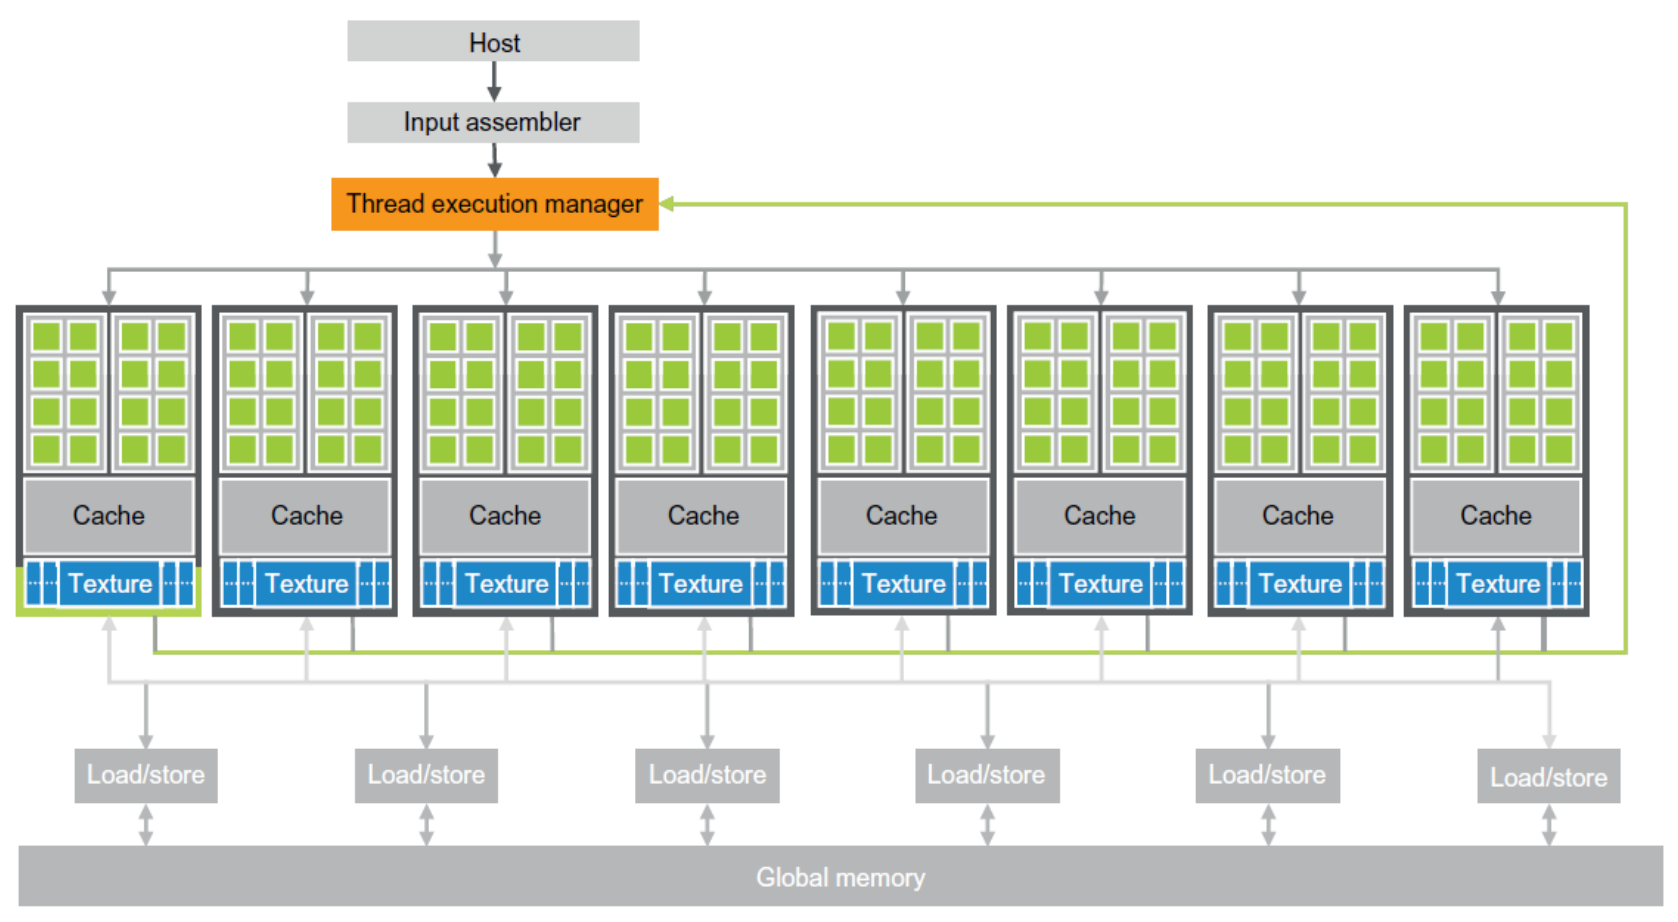
\includegraphics[width=.9\linewidth]{images/chapter2/cuda_arch.png}
    \caption{Architettura di una GPU CUDA-compatibile}
    \label{fig:cuda_arch}
\end{figure}


\section[CUDA e Vulkan]{CUDA e Vulkan}


Con il rilascio di CUDA, nel 2007, NVIDIA commercializza la prima GPU che riserva aree specifiche di silicio per semplificare la programmazione parallela. Questo non rappresenta solo cambiamenti software, ma vennero aggiunte componenti hardware ai chip stessi. Nei chip G80 e nei loro successori dedicati al calcolo parallelo, i programmi CUDA non attraversano più l'interfaccia grafica. Invece, una nuova interfaccia di programmazione parallela ad uso generale gestisce le richieste dei programmi CUDA. Questa interfaccia di programmazione espande notevolmente i tipi di applicazioni che è possibile sviluppare per le GPU. Inoltre, anche tutti gli altri strati software furono ridisegnati, consentendo ai programmatori di utilizzare i familiari strumenti di programmazione C/C++. Sebene sia ancora possibile usare la vecchia interfaccia di programmazione basata su OpenGL, l'avvento di CUDA e il supporto al computing da parte di Nvida ha reso molto più facile e piacevole sviluppare applicazioni parallele eliminando la necessità di utilizzare API grafiche.

Solamente un anno dopo Khronos Group, un consorzio industriale che gestisce lo sviluppo e la promozione di standard aperti, rilascia OpenCL, framework che fornisce una piattaforma aperta e standardizzata per la programmazione parallela su sistemi eterogenei. Così come CUDA, anche OpenCL mira a fornire una piattaforma unificata per lo sviluppo di applicazioni che possono sfruttare le capacità di elaborazione parallela, ma a differenza di CUDA, OpenCL supporta varie architetture hardware e non ha bisogno di chip dedidati. Un aspetto fondamentale di OpenCL è la sua natura di standard aperto e multi-piattaforma: ciò significa che gli sviluppatori possono scrivere codice OpenCL che può essere eseguito su una molteplici di dispositivi, indipendentemente dal produttore. OpenCL ha subito diverse revisioni nel corso degli anni per migliorare le funzionalità e la flessibilità. 

\begin{figure}[ht]
    \centering
    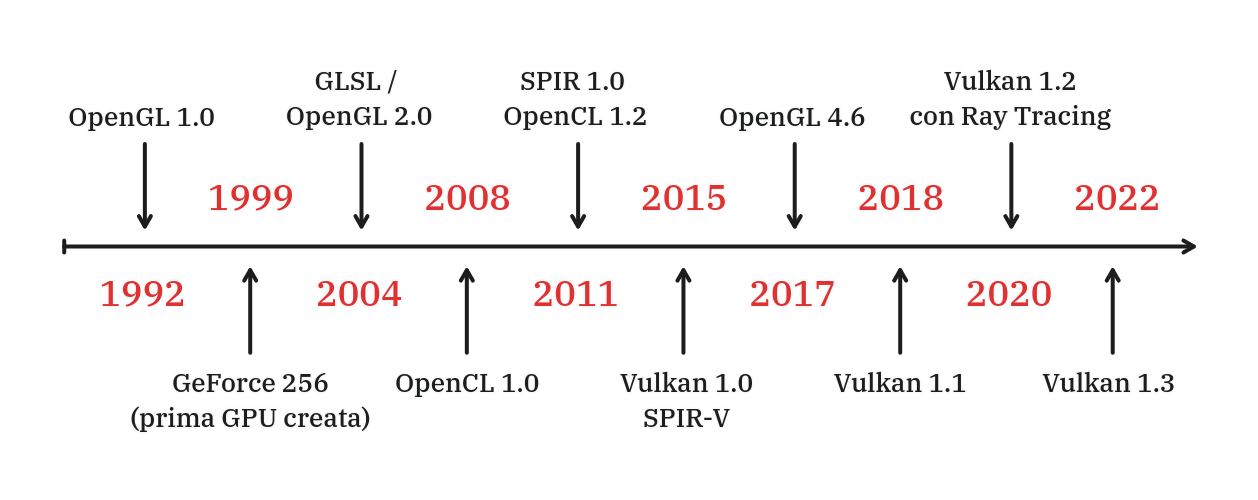
\includegraphics[width=.9\linewidth]{images/chapter2/vulkan_history.png}
    \caption{Contributi di Khronos Group}
    \label{fig:vulkan_history}
\end{figure}

Col tempo, Khronos Group ha riconosciuto la necessità di unire le caratteristiche di grafica e calcolo in un'unica API. Vulkan è stata sviluppata con l'obiettivo di superare le limitazioni di OpenGL e di fornire un accesso più diretto alle risorse hardware, consentendo una maggiore parallelizzazione e un controllo più fine da parte degli sviluppatori. Vulkan offre una serie di funzionalità che lo rendono più efficiente e flessibile rispetto ad OpenGL, inclusa una migliore gestione delle risorse, un controllo più diretto sulla GPU, una maggiore parallelizzazione e una minore overhead di driver. Vulkan è progettata per essere più adatta agli sviluppatori che richiedono il massimo delle prestazioni all'hardware, come nei giochi e nelle applicazioni di realtà virtuale. In sintesi, Vulkan rappresenta una naturale evoluzione di OpenGL e OpenCL, cercando di unire le migliori caratteristiche di entrambe per fornire un'API più potente, efficiente e adatta alle moderne architetture hardware. In fig. \ref*{fig:vulkan_history} è visibile l'evoluzione nel tempo delle API rilasciate da Khronos Group. Sia OpenGL che OpenCL sopravvivono tutt'oggi per la facilità di sviluppo delle applicazioni e l'ampio supporto hardware, sebbene siano meno performanti di CUDA e Vulkan.

\subsection[CUDA]{CUDA}

La struttura di un programma CUDA riflette la coesistenza di un host (CPU) e uno o più device (GPU) nel computer. Ogni file di origine CUDA può contenere sia di codice host che codice device. Per impostazione predefinita, qualsiasi programma C/C++ è un programma CUDA che contiene solo codice host. È possibile aggiungere funzioni e dichiarazioni di dati per il dispositivo in qualsiasi file di origine C/C++. Le dichiarazioni di funzioni o dati per il dispositivo sono chiaramente contrassegnate con particolari keyword di CUDA. Queste sono tipicamente funzioni che mostrano una grande quantità di parallelismo dei dati. Il codice deve essere compilato da un compilatore che riconosce e comprende queste dichiarazioni aggiuntive. Il compilatore CUDA ufficiale è NVCC (NVIDIA C Compiler) prodotto da NVIDIA.

\begin{figure}[ht]
    \centering
    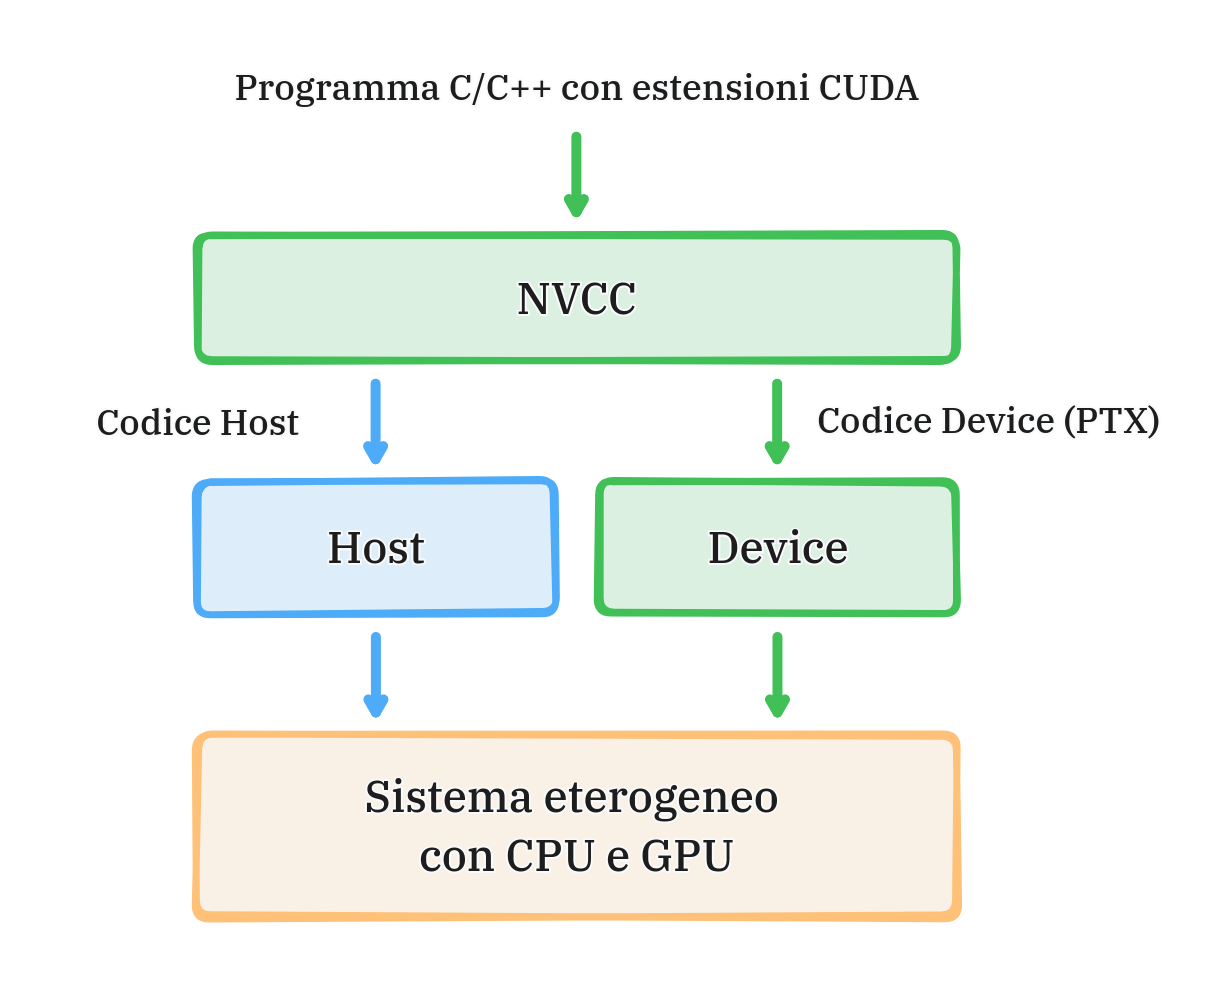
\includegraphics[width=.9\linewidth]{images/chapter2/nvcc.png}
    \caption{Processo di compilazione di un programma CUDA}
    \label{fig:nvcc}
\end{figure}

NVCC elabora il programma CUDA, utilizzando le keyword CUDA per separare il codice host e il codice device. Il codice host è codice normale ANSI C, che viene ulteriormente compilato con i compilatori standard C/C++ dell'host e viene eseguito come un processo CPU tradizionale. Il codice device è contrassegnato con le keyword CUDA per etichettare le funzioni di parallelismo dei dati, chiamate kernel, e le relative strutture di dati associate. Il codice device viene ulteriormente compilato da un componente runtime di NVCC ed eseguito su un device GPU. L'esecuzione inizia sull'host e quando una funzione kernel viene chiamata, essa viene eseguita da un gran numero di thread sul device. Tutti i thread generati da un avvio del kernel sono collettivamente chiamati una ``grid''.

\lstinputlisting[language=C++, caption=Somma di vettori in CUDA, label=lis:sum_vec]{code/cuda_example.cu} 

Il codice in \ref*{lis:sum_vec} mostra un programma cuda che somma due vettori parallelizzando su GPU. La keyword \verb|__global__| indica che la funzione è un kernel CUDA che verrà eseguita in ogni thread della `grid' della GPU. I vettori vengono create nella memoria host, copiati nella memoria device, elaborati e il risultato della computazione si troverà nel vettore \verb|res_vec| in memoria device, e dovrà essere ricopiato in memoria host per potervi accedere dai pezzi di codice C/C++. Le funzioni \verb|cudaMalloc|, \verb|cudaFree| e \verb|cudaMemcpy| sono le equivalenti del C++ \verb|malloc|, \verb|free| e \verb|memcpy|, e gestiscono l'allocazione di memoria device e la copia di memoria tra host e device.

\begin{figure}[ht]
    \centering
    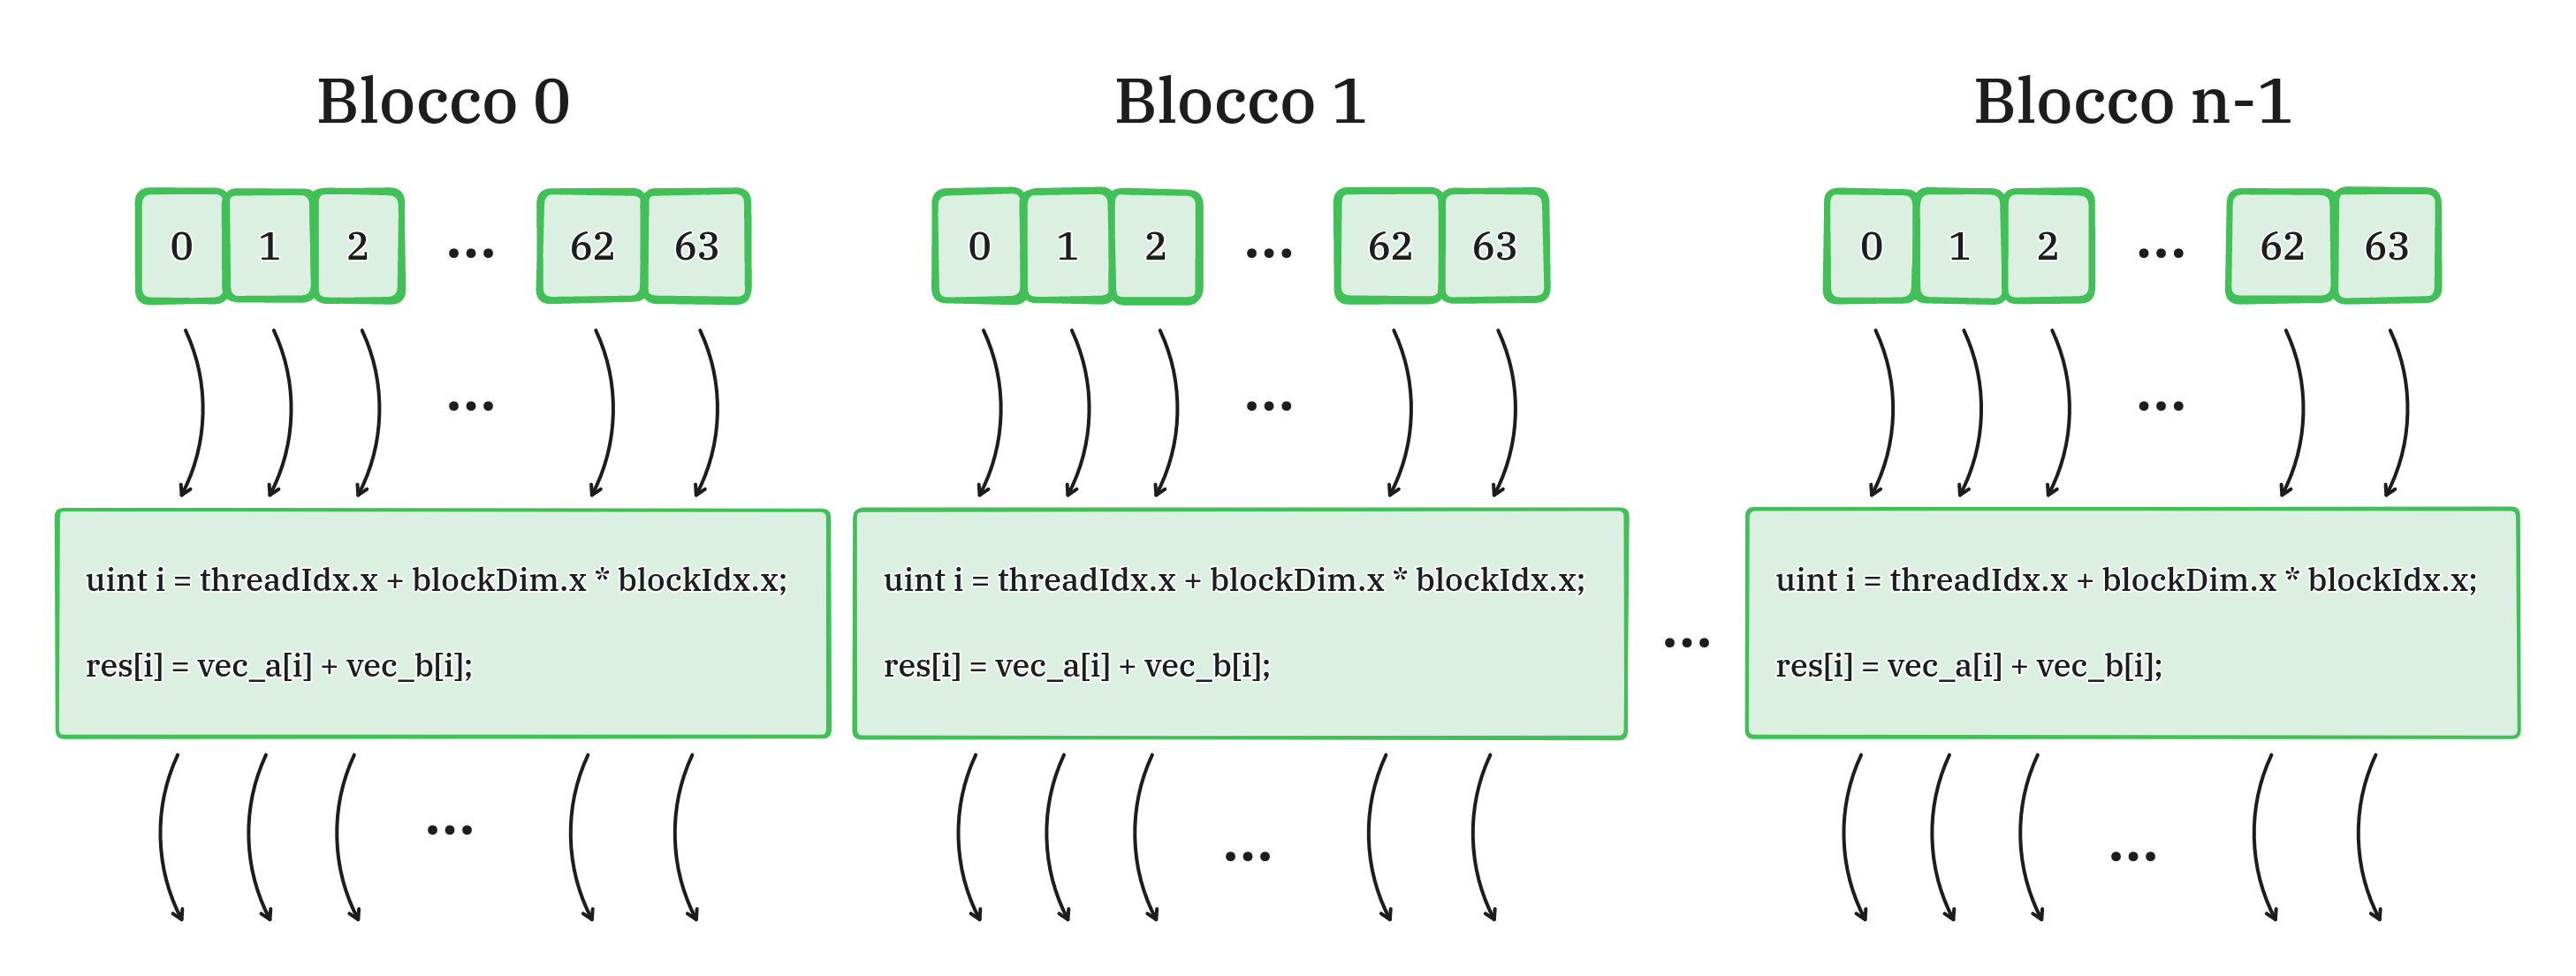
\includegraphics[width=.9\linewidth]{images/chapter2/grid.png}
    \caption{Processo di compilazione di un programma CUDA}
    \label{fig:grid}
\end{figure}


!! todo spiegare il kernel

\subsection[Vulkan]{Vulkan}
